\begin{figure}[htb!]
  \begin{subfigure}[b]{0.23\textwidth}
    \centering
    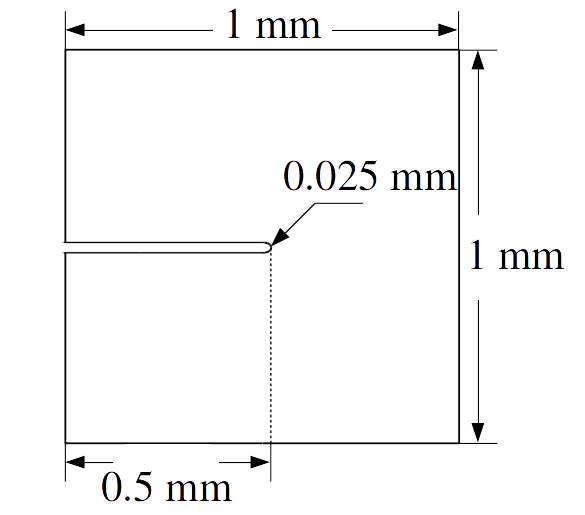
\includegraphics[width=\textwidth,scale=0.5]{Chapter4/figures/notched_plate_dimensions.png}
    \caption{}
  \end{subfigure}
  \begin{subfigure}[b]{0.21\textwidth}
    \centering
    
\includegraphics[width=\textwidth,scale=0.5]{Chapter4/figures/notched_plate_initial.png}
    \caption{}
  \end{subfigure}
  \begin{subfigure}[b]{0.21\textwidth}
    \centering
    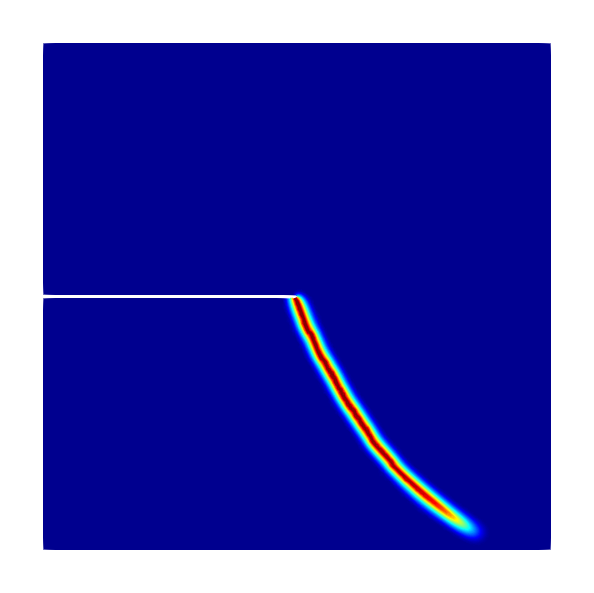
\includegraphics[width=\textwidth,scale=0.5]{Chapter4/figures/mode2_notched_plate_spectral_intermediate.png}
    \caption{}
    \label{fig: Chapter4/mode2_notched_plate_spectral_intermediate}
  \end{subfigure}
  \begin{subfigure}[b]{0.21\textwidth}
    \centering
    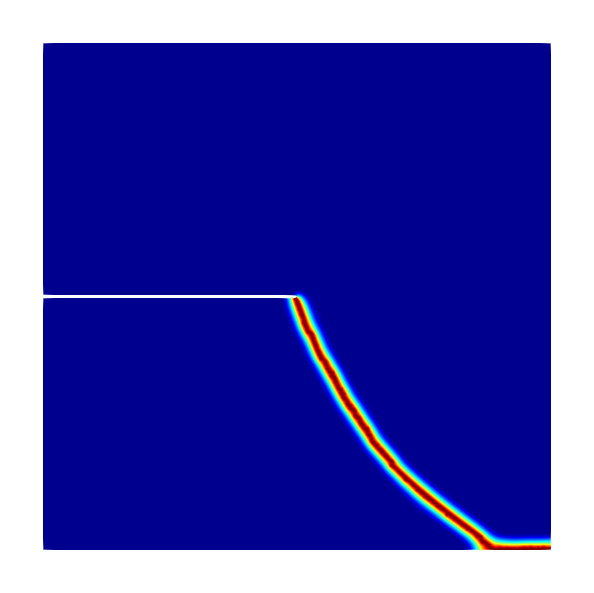
\includegraphics[width=\textwidth,scale=0.5]{Chapter4/figures/mode2_notched_plate_spectral_final.png}
    \caption{}
    \label{fig: Chapter4/mode2_notched_plate_spectral_final}
  \end{subfigure}
  \begin{subfigure}[b]{0.06\textwidth}
    \centering
    \caption*{d}
    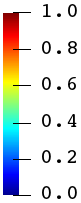
\includegraphics[width=\textwidth]{Chapter4/figures/jet_vertical.png}
    \vspace{0.15in}
  \end{subfigure}
  
  \hspace{0.015\textwidth}
  \begin{subfigure}[b]{0.21\textwidth}
    \centering
    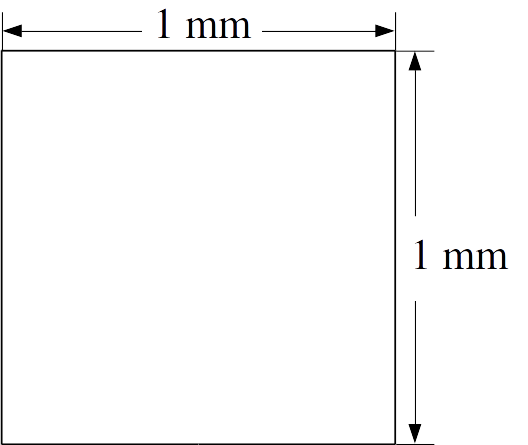
\includegraphics[width=\textwidth,scale=0.5]{Chapter4/figures/intact_plate_dimensions.png}
    \vspace{-0.03\textwidth}
    \caption{}
  \end{subfigure}
  \begin{subfigure}[b]{0.21\textwidth}
    \centering
    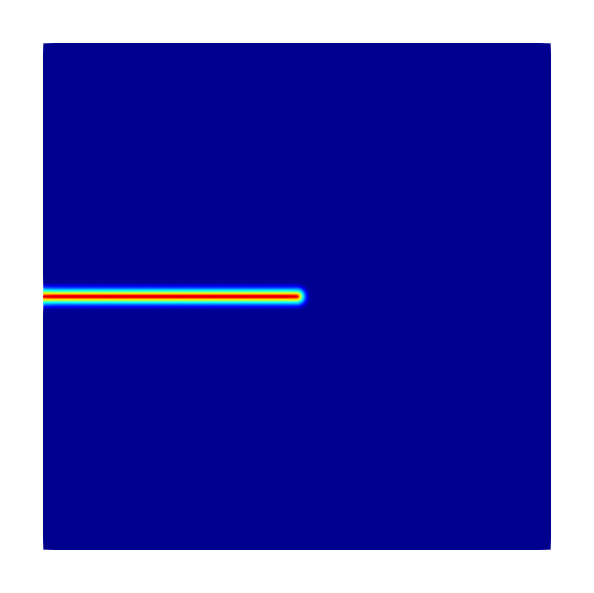
\includegraphics[width=\textwidth,scale=0.5]{Chapter4/figures/intact_plate_initial.png}
    \caption{}
  \end{subfigure}
  \begin{subfigure}[b]{0.21\textwidth}
    \centering
    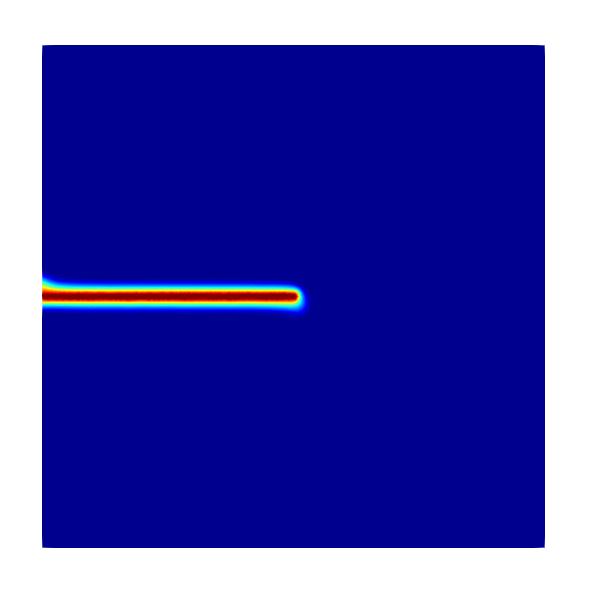
\includegraphics[width=\textwidth,scale=0.5]{Chapter4/figures/mode2_intact_plate_spectral_intermediate.png}
    \caption{}
    \label{fig: Chapter4/mode2_intact_plate_spectral_intermediate}
  \end{subfigure}
  \begin{subfigure}[b]{0.21\textwidth}
    \centering
    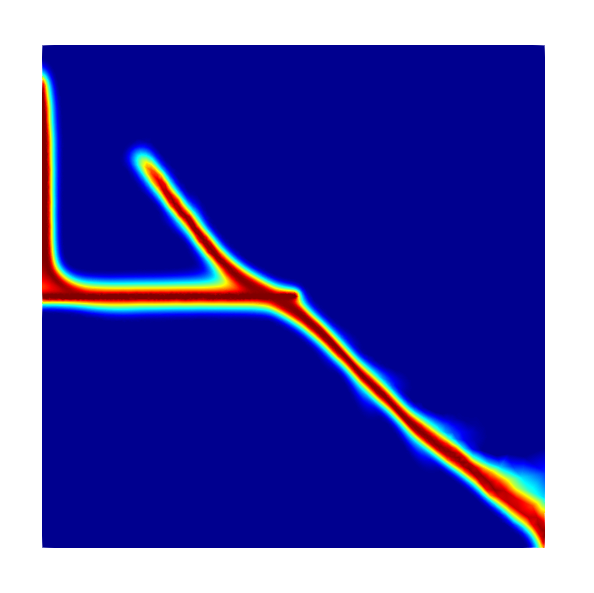
\includegraphics[width=\textwidth,scale=0.5]{Chapter4/figures/mode2_intact_plate_spectral_final.png}
    \caption{}
    \label{fig: Chapter4/mode2_intact_plate_spectral_final}
  \end{subfigure}
  \begin{subfigure}[b]{0.06\textwidth}
    \centering
    \caption*{d}
    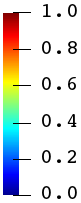
\includegraphics[width=\textwidth]{Chapter4/figures/jet_vertical.png}
    \vspace{0.15in}
  \end{subfigure}
  
  \hspace{0.015\textwidth}
  \begin{subfigure}[b]{0.21\textwidth}
    \centering
    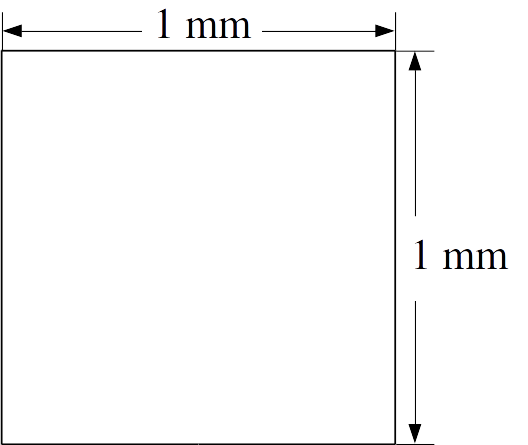
\includegraphics[width=\textwidth,scale=0.5]{Chapter4/figures/intact_plate_dimensions.png}
    \vspace{-0.03\textwidth}
    \caption{}
  \end{subfigure}
  \begin{subfigure}[b]{0.21\textwidth}
    \centering
    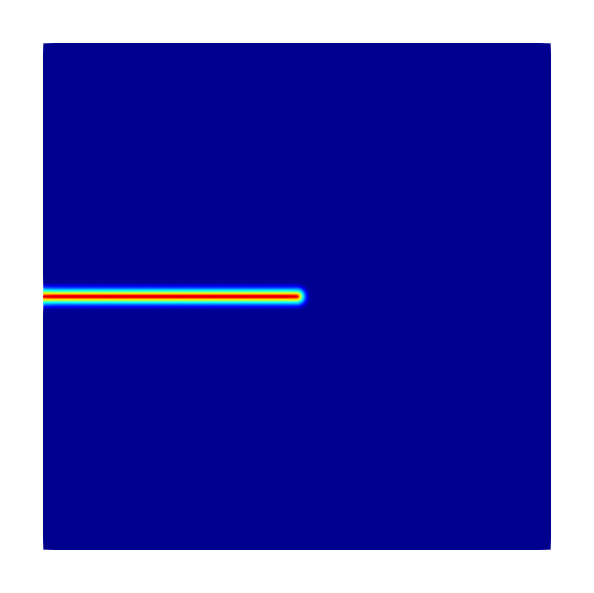
\includegraphics[width=\textwidth,scale=0.5]{Chapter4/figures/intact_plate_initial.png}
    \caption{}
  \end{subfigure}
  \begin{subfigure}[b]{0.21\textwidth}
    \centering
    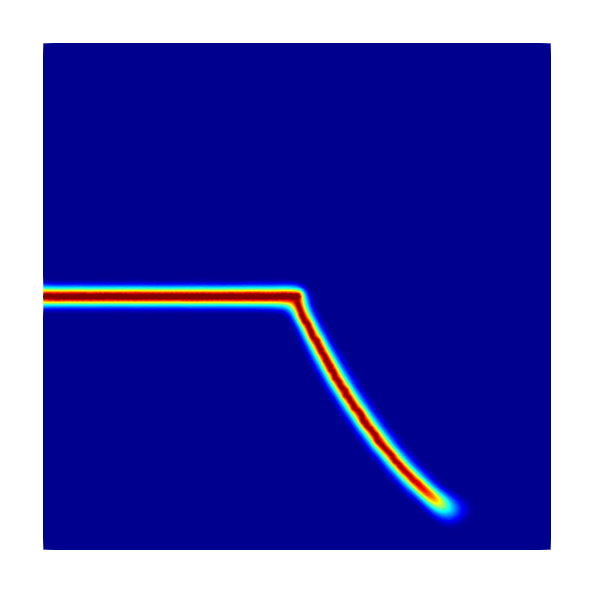
\includegraphics[width=\textwidth,scale=0.5]{Chapter4/figures/mode2_intact_plate_odd_intermediate.png}
    \caption{}
    \label{fig: Chapter4/mode2_intact_plate_odd_intermediate}
  \end{subfigure}
  \begin{subfigure}[b]{0.21\textwidth}
    \centering
    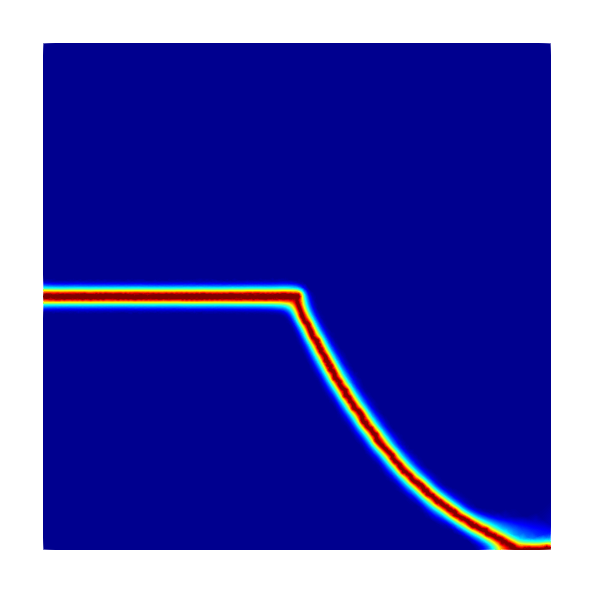
\includegraphics[width=\textwidth,scale=0.5]{Chapter4/figures/mode2_intact_plate_odd_final.png}
    \caption{}
    \label{fig: Chapter4/mode2_intact_plate_odd_final}
  \end{subfigure}
  \begin{subfigure}[b]{0.06\textwidth}
    \centering
    \caption*{d}
    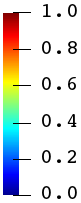
\includegraphics[width=\textwidth]{Chapter4/figures/jet_vertical.png}
    \vspace{0.15in}
  \end{subfigure}
  \caption[The crack paths for the Mode-II test.]{The crack paths obtained using (a-d) the spectral decomposition on a geometrically notched plate, (e-h) the spectral decomposition with an initial phase field $d_0$ \eqref{eq: mode1 initial damage} representing the initial crack, and (i-l) the contact split with an initial phase field. Snapshots of crack paths are shown at (b,f,j) $u_x = \SI{0}{\milli\meter}$, (c,g,k) $u_x = \SI{0.0109}{\milli\meter}$, and (d,h,l) $u_x = \SI{0.02}{\milli\meter}$. }
  \label{fig: Chapter4/mode2_crack_path}
\end{figure}
